\chapter{A Tutorial Game}
\label{ch:tutorial_game}
As the second part of my own work, I designed and implemented a prototype for an educational game for \gls{uml} Activities in the context of Reactive Blocks, nicknamed simply \emph{The Reactive Blocks Game}. Based on the tutorial described in Ch.~\ref{ch:reactive_blocks_tutorial}, this game teaches the same concepts in similar ways, but in a different environment. This chapter covers the motivation for creating the game, as well as a description of the design and implementation of the prototype. Additionally, a user test was conducted in an effort to uncover usability issues with the game prototype.

\section{Motivation}
\label{sec:game_motivation}

\subsection{Goals}
\label{sec:game_goals}
Like with the tutorial in Ch.~\ref{ch:reactive_blocks_tutorial}, I initially set some goals for the design and implementation of the game. These goals are primarily based on experiences from the tutorial implementation and test, as well as the good practices from Sect.~\ref{sec:good_practices_games}.

\paragraph{Immersion} The primary goal for the game is to provide an environment where players can immerse themselves in the learning experience. This involves giving the players a sense of identity within the game, and providing them with challenges that are easily visualized and comprehended (but not necessarily solved) within the given environment.

\paragraph{Exploration and Guidance} \gls{uml} Activities can be used to model very complex systems, and learning how to do this is not a trivial process. The game is thus likely to benefit from providing some guidance to players, as opposed to complete freedom to explore~\cite{andersen:tutorials_impact}. Some freedom is still necessary, to facilitate creativity and deeper learning~\cite{bonawitz:double_edged_pedagogy}. The goal is then that the game should be primarily focused around a tutorial-like guided path for learning about concepts within \gls{uml} Activities, but with the possibility for players to find their own solutions to problems. Players should also be encouraged to explore other perspectives, and maybe find different or even \emph{better} solutions to the same problems.

\paragraph{Level of Difficulty} The target audience for the game is people who want or need to learn about software modeling with \gls{uml}, which is likely to be a fairly small group of people (in the big picture). However, these people often come with different backgrounds: some may be experienced programmers looking for a way to visualize their programs, while others are people without any previous experience dealing with software structures. The game should be easy enough for the less knowledgeable users to get started without frustration, but eventually provide challenges that feel relevant also to the more experienced. Players should also have the option to skip challenges they feel are less relevant or that involve concepts they have already mastered, in order to avoid the game experience becoming tedious.

\paragraph{Lessons from the Tutorial} The design and implementation of the tutorial in Ch.~\ref{ch:reactive_blocks_tutorial} fulfilled some, but not all of the goals that were set. The approach seemed to provide a decent learning experience, but with some potential for improvement. A goal for the game is to build on the parts of the tutorial that were successful, such as the teaching order, and additionally include some of the parts that were not implemented, such as having everything in one place. Since the game still will be based on Reactive Blocks, many of the same challenges will be present, but with a game, there should be more options for providing resources within the same platform, such as help-on-demand.

\section{Concept Development}
\label{sec:game_concept}
When developing the concept of the game, a few points were considered. First of all, it should involve some sort of main character, giving the player a sense of identity. Secondly, the game concept must accommodate a range of different types of challenge that are suited for learning about concepts like concurrency, modularization and reuse. Finally, it must be relatively easy to prototype, as the available time to implement the game was fairly limited.

\subsection{The Final Concept}
\label{sec:game_final_concept}
With the above design points in mind, I settled on a two-dimensional maze-navigating game, where the player controls a character or set of characters through operations and logic in Reactive Blocks. The main character, Malcolm, must perform one or more goals to complete the level, such as gathering stars. In order to get to these stars however, Malcolm must perform some other tasks, such as gathering keys, or invoke the assistance of other characters in the game. Figure~\ref{fig:level3map} shows level 3 of the game, where Malcolm must navigate around the maze and gather all four stars.

\begin{figure}[htp]
	\centering
	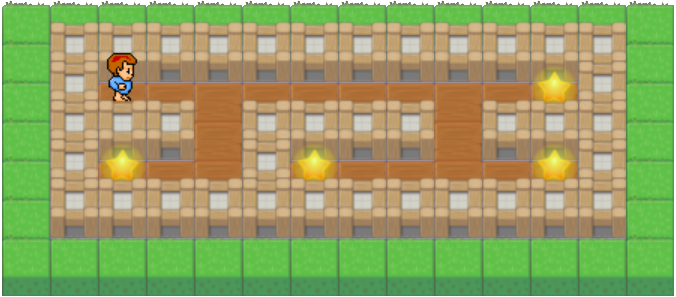
\includegraphics[scale=0.60]{level3map}
	\caption[Level 3 of the Reactive Blocks game]{Level 3 of the Reactive Blocks game. Malcolm, the character on the left, must move around the maze and collect all four stars in order to complete the level.}
	\label{fig:level3map}
\end{figure}

\noindent
This concept was chosen for the following reasons:
\begin{itemize}
	\item Two-dimensional games are quick and easy to implement, both graphically and programming-wise, given an appropriate framework.
	\item Since the purpose of the game is to teach \gls{uml} Activities, it makes most sense to provide a game environment where the player must program their characters' path in advance, and then see if they modeled the desired behavior correctly. A two-dimensional maze-navigating game makes it easy for players to get a clear overview of what they are supposed to do.
	\item Despite being relatively simple to implement, a two-dimensional maze-game offers a lot of possibilities in the form of obstacles and challenges the player must overcome in order to complete each level.
\end{itemize}

\noindent
Even with such a flexible concept in place, it was no trivial task to create levels and challenges that let the user learn about \gls{uml} Activity concepts in an intuitive and reasonable way. In addition, I had to consider how each concept should be introduced within the level, so that the user would know what to expect.

\subsection{The Tutorial Part}
\label{sec:game_tutorial}
One of the most important goals for the game was to provide an environment where the player could find all the information needed to complete a level, instead of having to switch between contexts or search through external sources. Players would be creating the logic for each level in Reactive Blocks, generate code from these models, and run it to see if it was correct. Thus, additional information, such as concept introductions, level maps, and help-on-demand, had to be presented inside Reactive Blocks. Unfortunately, because I was unable to alter the Reactive Blocks environment, I could still not provide a tutorial mode, just as with the tutorial in Ch.~\ref{ch:reactive_blocks_tutorial}.

\noindent
Instead of a tutorial mode in Reactive Blocks, a different solution presented itself. I could create a separate program with a window that would contain the most basic information needed for each level, with internal links to additional resources. This would of course not be completely within the context of Reactive Blocks, but hopefully a decent substitute for the lack of a real tutorial mode.

\noindent
Designing the tutorial window presented some challenges of its own. The window needed to be small enough for players to be able to keep it on their screen together with the Eclipse/Reactive Blocks window, preferably also for smaller screens like on laptops. At the same time, I needed to include all the info a player would realistically need to complete each level. Obviously I would not be able to fit all the information in one small window at the same time, so I had to decide which elements to display by default, and what should only be displayed upon the player's request.

\noindent
After some consideration, I settled on a 600x800 pixels window, which should fit pretty good with the Reactive Blocks modeling canvas on screen resolutions down to 1280x800. When the resolution becomes smaller than this, there is little room for anything but the Eclipse window anyway. Given more time for development, it would likely be better to have a variable size window depending on the available screen resolution, but for now, this size is fixed.

\noindent
Figure~\ref{fig:level1_intro} shows the introduction window for level 1. The layout is the same for all levels, but the content varies. At the top is simply the title of the level, with a ``tagline'' giving a short description of what the current level is about. Below the title is a slide show, which the player may go through to get a quick introduction of the concepts taught by, and the goals of, the current level. These introductions are generally kept short, except for in level 1, where the whole game must be introduced in additional to all the most basic concepts. The player controls the slide show with the arrow and play/pause buttons.

\begin{figure}[htp]
	\centering
	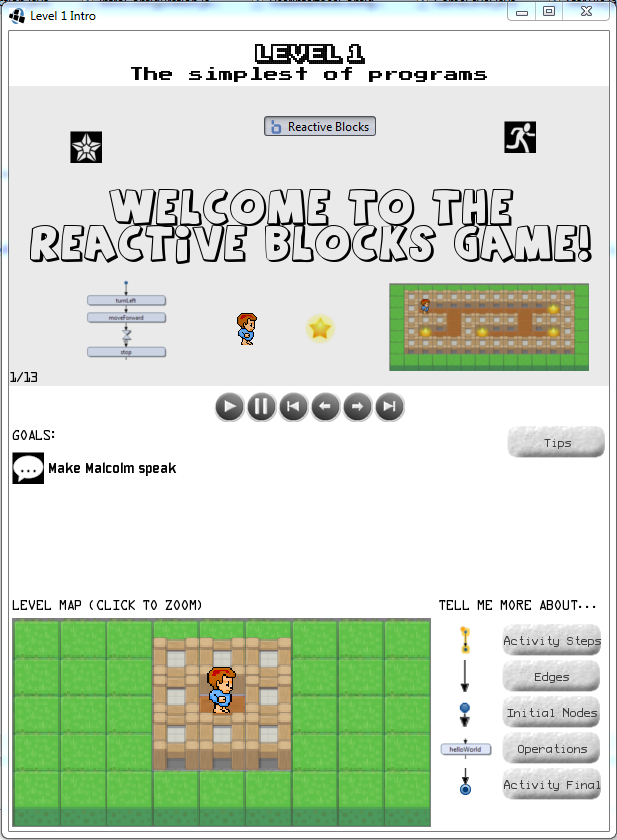
\includegraphics[scale=0.50]{level1_intro}
	\caption[Introduction window for level 1]{The introduction window for level 1, with the introduction slide show at the top, followed by the goals for this level, a button for tips, the level map, and some buttons for retrieving additional information about the concepts presented.}
	\label{fig:level1_intro}
\end{figure}

\noindent
Below the slide show, we see a list of the goals for the current level. The goals, together with the level map at the bottom, is the most important information of the level. The level map and the goals are always visible, so that the user has easy access to these when working on the solution for the current level. The level map varies in size, but is always scaled to fit the small frame in the bottom left corner. However, since the player sometimes has to check details of the map, it is possible to make it bigger by clicking on it.

\noindent
Finally, the buttons on the right side of the window represent the \emph{help-on-demand} information that is not visible by default. The \emph{Tips} button provides some tips that are good to know either for solving the current level, or for learning about modeling in general. The hope is that if players get stuck or are unsure about how to proceed, they will see and click this button in an attempt to find help. The \emph{Tell me more about...} buttons provide more detailed information about each concept presented in the current level, available for players who need more information in order to understand the concepts sufficiently, or simply want to learn more.

\noindent





\subsection{Game Levels}
\label{sec:game_levels}
For the first version of the prototype, only 5 levels were designed and implemented. This was because I wanted to test the prototype with a few users as soon as possible, in order to uncover any serious flaws with the \gls{ui} or the way the introductions were presented as early as possible. The levels for the first version of the prototype are briefly described below.

\subsubsection{Level 1}

\subsubsection{Level 2}

\subsubsection{Level 3}

\subsubsection{Level 4}

\subsubsection{Level 5} 

\section{Implementation}
\label{sec:game_implementation}


\section{User Testing and Feedback}
\label{sec:game_testing}


\subsection{Subject 1}
\label{sec:game_testing_subject1}

\subsubsection{Profile}

\subsubsection{Observations}

\subsubsection{Feedback}


\subsection{Subject 2}
\label{sec:game_testing_subject2}

\subsubsection{Profile}

\subsubsection{Observations}

\subsubsection{Feedback}


\subsection{Subject 3}
\label{sec:game_testing_subject3}


\subsubsection{Profile}

\subsubsection{Observations}

\subsubsection{Feedback}

\subsection{A Side-note on an Informal Experiment}
\label{sec:game_testing_sidenote}
In addition to the formal usability tests conducted with the three volunteer subjects, I thought it might be interesting to test the game experience on someone completely outside the target audience, just to see what happened. I decided my girlfriend, an elementary school English teacher with no experience even remotely related to programming (she does not like working with computers), would be a suitable subject.

\noindent
The experiment was conducted in an informal way, where she would simply do her best to absorb the information provided in the introductions, and then try to solve the exercises. I helped with some of the parts that were more technical and less relevant, such as preparing Eclipse and Reactive Blocks, and building and running the blocks. If she got completely stuck, I would also offer some hints, primarily about where she could find more information.

\noindent
To my slight surprise, my girlfriend actually handled the problems presented very well. She read the introductions carefully, and easily understood the concepts of operations, tokens and control flow. She handled timers without trouble, struggled a little with decisions (I had to explain what \emph{Strings}, \emph{booleans}, and \emph{integers} were), and used \emph{Merge} nodes perfectly to simplify the logic in level 5. She did spend notably more time on each level than the three subjects in the formal tests (she even got a little more help with \gls{ui} issues), but this could simply be because she was not used to building this particular kind of mental models, added to the fact that she read the instructions extra carefully.

\noindent
Despite her aversion for working with computers and lack of interest for software development, she found the game fun to play because it let her get the sense of mastering a skill she thought was far beyond her abilities. When starting both level 4 and 5, she sighed and exclaimed that \emph{``it looks really difficult''}, but attacked the problems with determination, reading and re-reading the introductions until things started to make sense.

\noindent
I should also include that while my girlfriend was able to understand the concepts presented sufficiently to solve problems within the context of the game, she admitted to having no idea about how they could be used for other purposes.

\noindent
While I found this experiment to be quite interesting, its informal nature prevents me from drawing any real conclusions. It is likely that a large part of my girlfriend's motivation was to support my thesis work, as opposed to wanting to learn about \gls{uml} Activities. Also, despite not having any interest in working with computer-related topics, she could simply be the type of person who has a knack for understanding these things (without even knowing it). All in all, much is left to speculation, but the experiment provides an interesting anecdote for the potential of educational games.

\section{Evaluation of the Tutorial Game}


